\documentclass[tikz,border=0pt]{standalone}
\usepackage{lmodern}
\usetikzlibrary{arrows.meta}
\definecolor{badge}{HTML}{2CA02C}
\definecolor{surface}{HTML}{E5F4E5}
\definecolor{front}{HTML}{80B880}
\definecolor{side}{HTML}{599559}
\definecolor{beam}{HTML}{000000}
\begin{document}
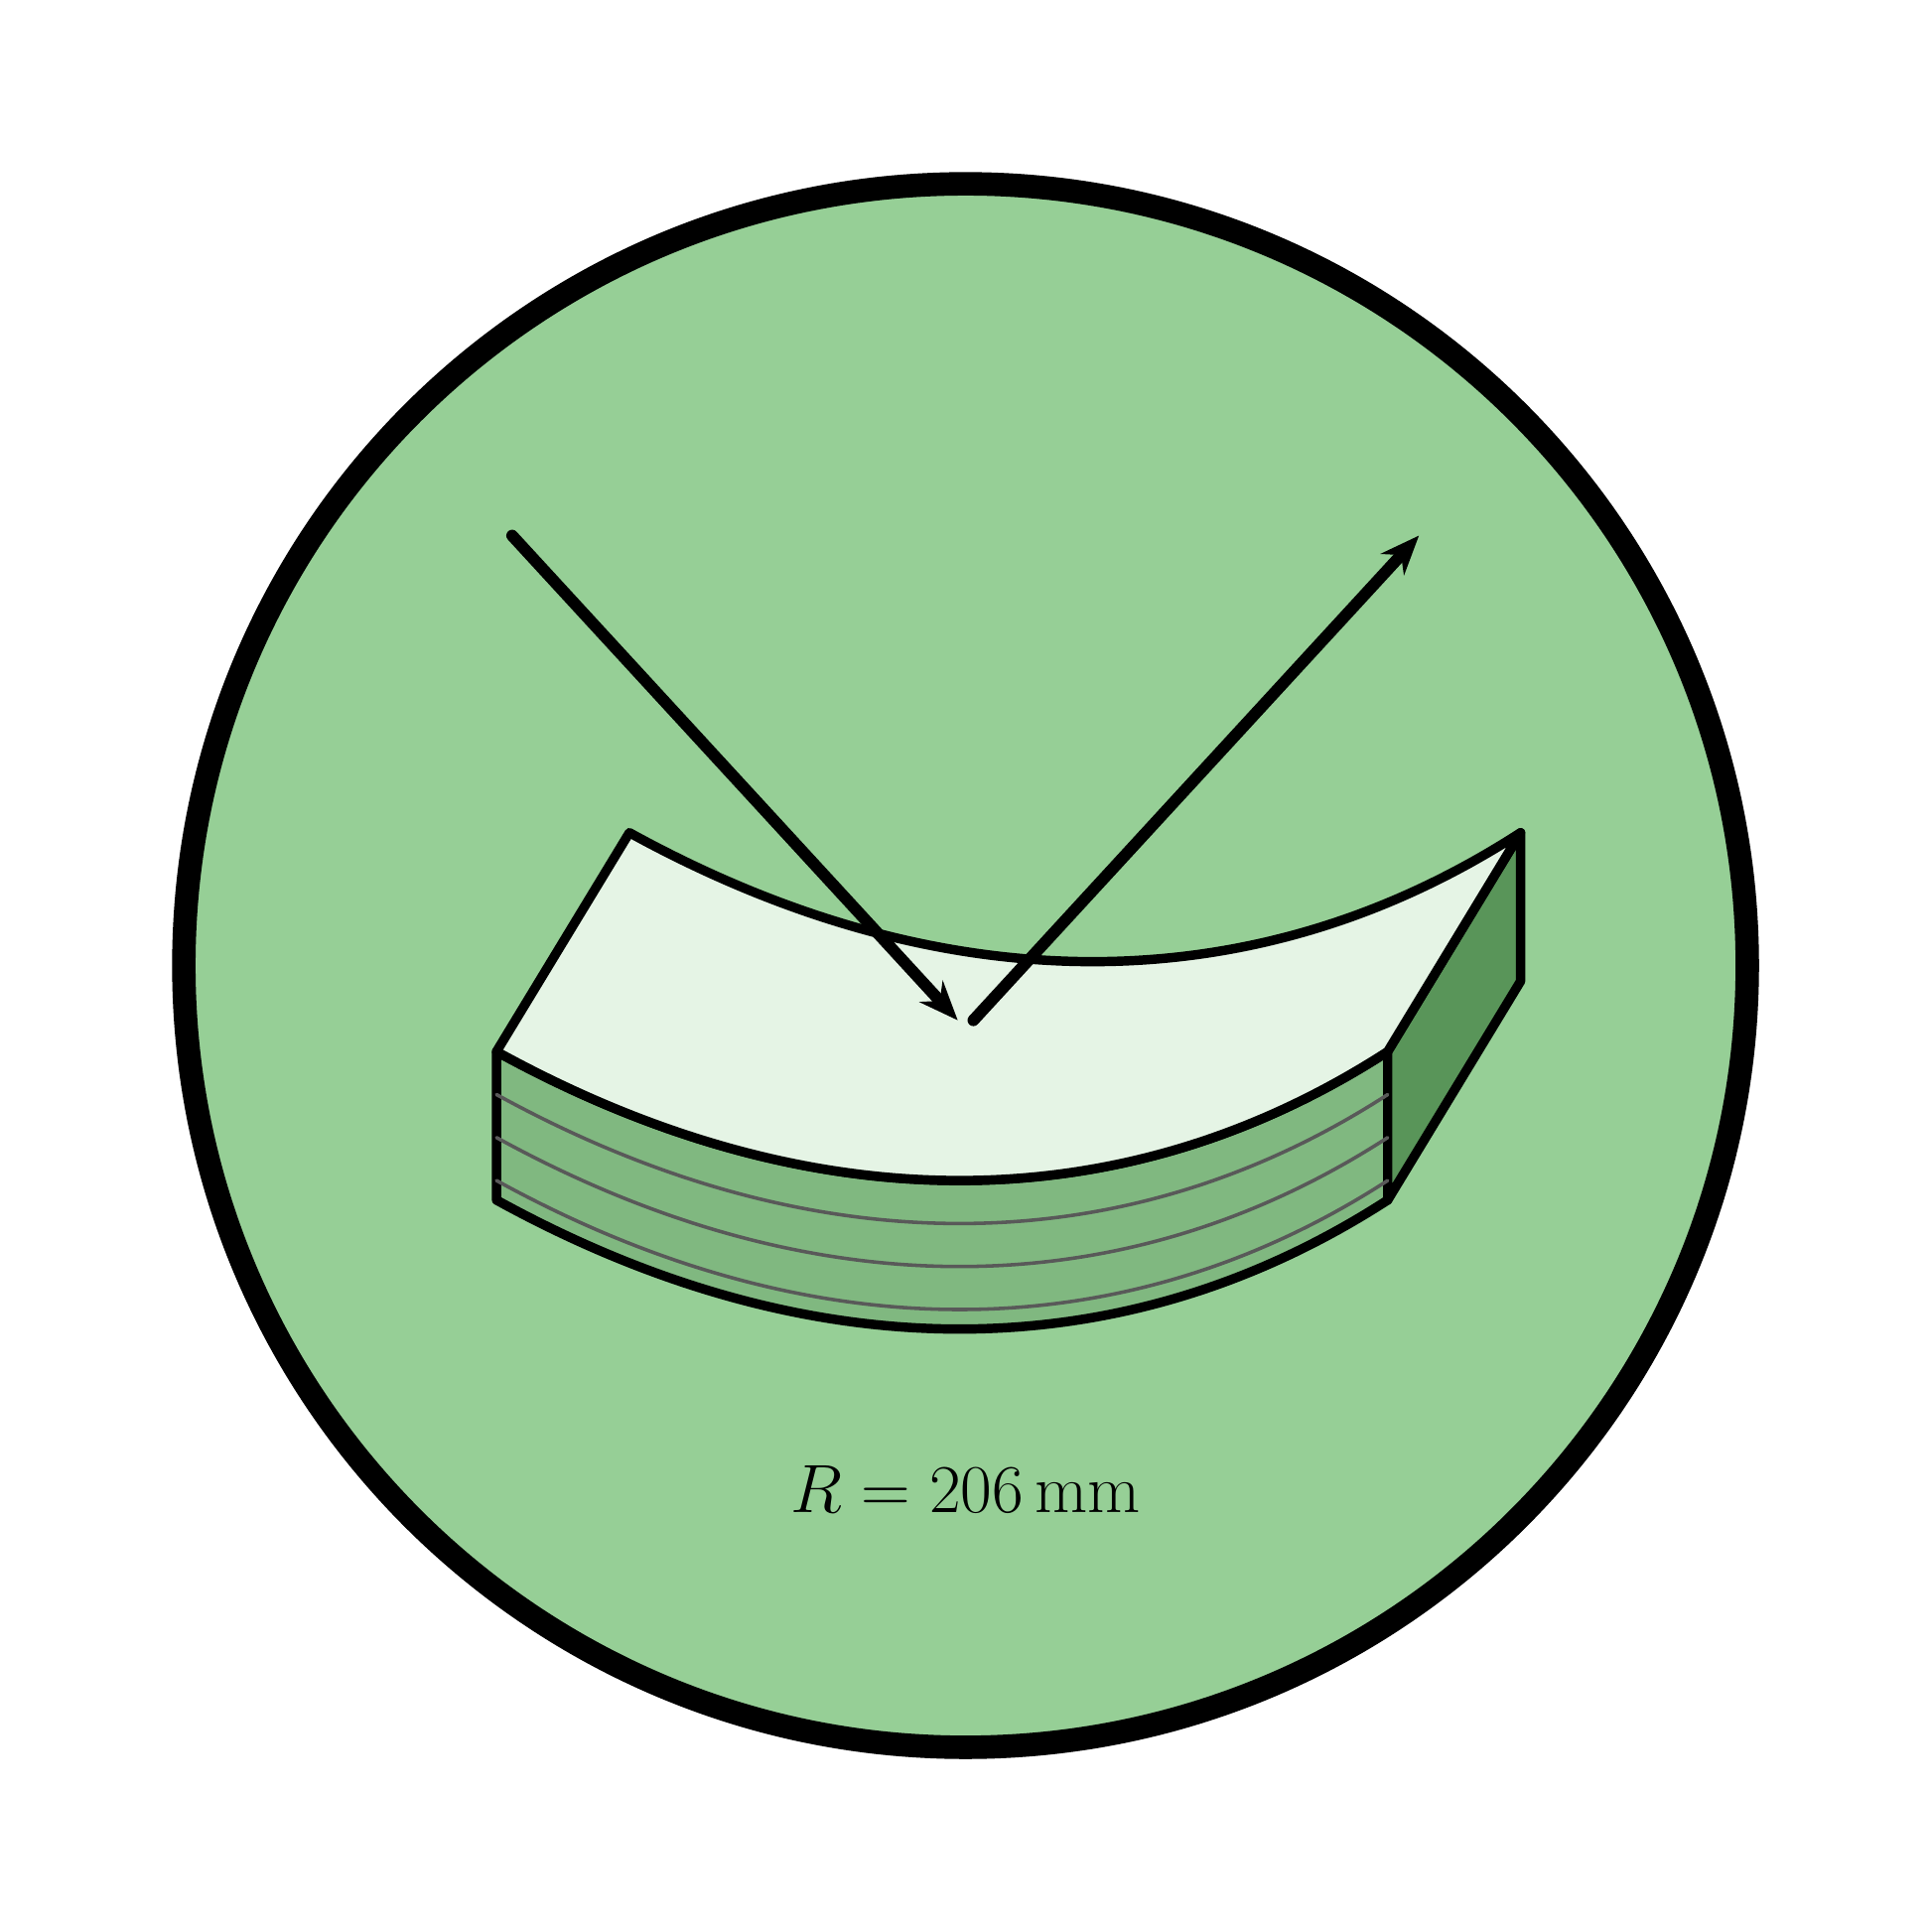
\begin{tikzpicture}[x=10mm,y=10mm,line cap=round,line join=round]
  \path[use as bounding box] (-12,-12) rectangle (12,12);
  \filldraw[fill=badge!50!white,draw=black,line width=3mm] (0,0) circle (10);
  % Schematic cylindrical substrate. Curvature exaggerated for legibility.
  % O-2094 specifies a 52 x 27 mm aluminium substrate with R = 206 mm.
  % This is neither a dimensioned drawing nor an optical ray trace.
  \begin{scope}[yshift=-8mm]
    % Front face and right end face.
    \path[fill=front,draw=black,line width=1.2mm]
      (-6,-.3) .. controls (-2,-2.5) and (2,-2.5) .. (5.4,-.3)
      -- (5.4,-2.2) .. controls (2,-4.4) and (-2,-4.4) .. (-6,-2.2) -- cycle;
    \path[fill=side,draw=black,line width=1.2mm]
      (5.4,-.3) -- (7.1,2.5) -- (7.1,.6) -- (5.4,-2.2) -- cycle;
    % Bent reflecting surface, translated along its cylinder axis.
    \path[fill=surface,draw=black,line width=1.2mm]
      (-6,-.3) .. controls (-2,-2.5) and (2,-2.5) .. (5.4,-.3)
      -- (7.1,2.5) .. controls (3.7,.3) and (-.3,.3) .. (-4.3,2.5) -- cycle;
    % Parallel curved lines suggest crystallographic planes / bent coating.
    \foreach \dy in {.55,1.1,1.65} {
      \draw[black!65,line width=.45mm]
        (-6,{-0.3-\dy}) .. controls (-2,{-2.5-\dy}) and (2,{-2.5-\dy}) .. (5.4,{-0.3-\dy});
    }
    % Symmetric beams only convey energy selection by diffraction.
    \draw[beam,line width=1.5mm,-{Stealth[length=5mm,width=4mm]}]
      (-5.8,6.3) -- (-.1,.1);
    \draw[beam,line width=1.5mm,-{Stealth[length=5mm,width=4mm]}]
      (.1,.1) -- (5.8,6.3);
  \end{scope}
  \node[font=\fontsize{32}{38}\selectfont] at (0,-6.7) {$R=206\,\mathrm{mm}$};
\end{tikzpicture}
\end{document}
